\chapter{Evaluation}
\section{Bewertungskriterien}
\subsection{Diskriminator-Verlust}
Der Diskriminator-Verlust ist ein wesentliches Maß für die Effektivität des Diskriminators in einem GAN-Modell. Ein niedriger Diskriminator-Verlust bedeutet, dass der Diskriminator erfolgreich zwischen echten und generierten Bildern unterscheiden kann. Im Kontext eines GANs zeigt ein abnehmender Diskriminator-Verlust über die Epochen hinweg, dass der Diskriminator zunehmend besser darin wird, die Authentizität der Bilder zu beurteilen. Ein hoher Diskriminator-Verlust weist hingegen darauf hin, dass das Modell Schwierigkeiten hat, echte von generierten Bildern zu unterscheiden, was ein Indikator für Verbesserungspotenzial im Training oder der Modellarchitektur sein könnte.

\subsection{Generator-Verlust}
Der Generator-Verlust ist ein Indikator für die Fähigkeit des Generators, Bilder zu erzeugen, die vom Diskriminator als echt eingestuft werden. Ein hoher Generator-Verlust deutet darauf hin, dass der Generator die realen Daten noch nicht effektiv nachahmen kann, während ein niedriger Generator-Verlust ein Zeichen dafür ist, dass die generierten Bilder den echten immer ähnlicher werden. Im Verlauf des Trainings sollte der Generator-Verlust tendenziell abnehmen, was darauf hindeutet, dass der Generator lernt, überzeugendere Bilder zu produzieren.

\subsection{Diskriminator Genauigkeit}
Die Diskriminator-Genauigkeit gibt an, wie oft der Diskriminator korrekt zwischen echten und gefälschten Bildern unterscheidet. Eine hohe Genauigkeit bedeutet, dass der Diskriminator effektiv arbeitet, während eine niedrige Genauigkeit auf Probleme bei der Unterscheidung hinweisen kann. Es ist wichtig, ein Gleichgewicht zu finden, denn eine zu hohe Genauigkeit kann darauf hindeuten, dass der Diskriminator die generierten Bilder zu leicht erkennt, was auf ein Problem mit dem Generator hinweisen könnte.\newline
In einem ideal funktionierenden GAN sollte der Diskriminator eine Genauigkeit von etwa 50$\%$ erreichen. Das bedeutet, dass der Diskriminator die echten von dem generierten Bildern nur zufällig unterscheiden bzw. nicht mehr zuverlässig unterscheiden kann, was zeigt dass das GAN gut trainiert wurde.

\subsection{SSIM-Score (Structural Similarity Index)}
Der SSIM-Score ist ein Maß für die visuelle Ähnlichkeit zwischen den generierten Bildern und den entsprechenden Originalbildern. Er bewertet die Bildqualität anhand von Faktoren wie Helligkeit, Kontrast und Struktur. Ein hoher SSIM-Wert deutet darauf in, dass die generierten Bilder den echten Bildern sehr ähnlich sind, was ein Zeichen für eine hohe Bildqualität ist. Ein niedriger SSIM-Wert kann auf deutliche Unterschiede in der visuellen Struktur hinweisen, was Verbesserungsbedarf im Generator-Training oder in der Modellarchitektur signalisiert.

\section{Ergebnisse und objektive Bewertung}
In diesem Abschnitt liegt der Fokus auf der objektiven Bewertung der Leistung des CycleGAN-Algorithmus. Es werden verschiedene Metriken und Kriterien herangezogen, um eine umfassende Bewertung durchzuführen, einschließlich der Verluste der Generatoren und Diskriminatoren bei Variation der Hyperparameter. Darüber hinaus wird eine detaillierte Analyse der Genauigkeit der Diskriminatoren und des SSIM-Scores durchgeführt. Diese Messungen sind sowohl für die genaue Bestimmung der Qualität der generierten Ergebnisse als auch für die Bewertung der Lernfähigkeit der Modelle von Bedeutung.

Die verwendeten Datensätze für die Evaluierung stammen aus dem Berkeley-Repository. Besondere Beachtung wird dem 'maps'-Datensatz geschenkt, bei dem Transformationen zwischen Kartenansichten und Satellitenbildern durchgeführt wurden. Das Training wurde mehrmals mit verschiedenen Hyperparameter-\\Konfigurationen durchgeführt, wobei Parameter wie der Lambda-Wert, die Anzahl der Epochen und die Lernrate des Optimizers variiert wurden. Ziel ist es, eine Konfiguration zu finden, bei der die Qualität der erzeugten Bilder nahe an der Qualität des Originals und die Leistung des Diskriminators optimal ist.

Die subjektive Bewertung erfolgt durch die visuelle Beurteilung der generierten Bilder aus dem Testdatensatz hinsichtlich stimmiger Farben, Struktur und Rauschen im Vergleich zu den Originalbildern. Darauf aufbauend erfolgt eine objektive Bewertung mithilfe der definierten Metriken.


\subsection{Pix2Pix}
Die Entwicklung eines Pix2Pix GANs stellt eine große Herausforderung dar, insbesondere im Hinblick auf das Training des Modells. Eine der zentralen Schwierigkeiten besteht darin, ein angemessenes Gleichgewicht zwischen effektivem Lernen und der Vermeidung von Overfitting zu finden. Overfitting tritt auf, wenn das Modell zu stark an die spezifischen Muster und Merkmale des Trainingsdatensatzes angepasst wird, was dazu führt, dass der Generator Probleme beim Übersetzen von unbekannten Daten hat. Dieses Problem tritt oft in Szenarien auf, in denen mit einem begrenzten Datensatz trainiert wird, wie in diesem Fall.\newline
In der praktischen Anwendung des Pix2Pix-Modells, das in diesem Fall speziell für die Transformation von Satellitenbildern in Karten entwickelt wurde, ist aufgefallen, dass der Generator besonders effizient bei der Erzeugung von Straßenlinien ist. Dies deutet auf eine starke Fähigkeit des Modells hin, lineare, kontrastreiche Strukturen zu erkennen und wiederzugeben.
Jedoch stößt das Modell an seine Grenzen, sobald es um die Darstellung von Farben und komplexeren Strukturen geht, insbesondere bei Grünflächen oder Wasser. Bei der Generierung dieser Elemente zeigt der Generator deutliche Schwierigkeiten, was sich in einer weniger präzisen und oft fehlerhaften Darstellung widerspiegelt. Die Beobachtungen ergaben, dass obwohl diese Elemente oftmals nur einen geringen Teil des Gesamtbildes ausmachen, sie dennoch einen großen negativen Einfluss auf das Gesamtergebnis haben.

Für das Training des Pix2Pix-Modells wurde der Adam-Optimierer mit einer initialen Lernrate von 0.0002 und den Momentum-Parametern $\beta$1 = 0.5 und $\beta2$ = 0.999 eingesetzt. Diese Einstellungen erweisen sich als effektiv, um einen guten Kompromiss zwischen Lerngeschwindigkeit und Stabilität des Trainingsprozesses zu ermöglichen. Eine Batchgröße von 1 wurde gewählt, um die Trainingseffizienz zu maximieren und qualitativ hochwertigere Ergebnisse zu erzielen. Während verschiedener Testdurchläufe konnte beobachtet werden, dass eine größere Batchgröße zwar das Training beschleunigt, jedoch zu schlechteren Trainingsergebnissen führt. Der Hyperparameter $\lambda$ wird genutzt, um das Gewicht des L1-Verlusts im Generatorverlust zu steuern und die Inhaltsähnlichkeit zwischen den generierten und den Zielbildern zu regulieren. Insgesamt hat das Modell eine Trainingsdauer von 100 Epochen durchlaufen, wobei die ersten 80 Epochen mit $\lambda$ = 100 und die restlichen 20 mit $\lambda$ = 150 absolviert wurden.

\begin{figure}[ht]
	\begin{subfigure}[t]{.14\textwidth}
		\centering
		\caption*{Eingabe}
		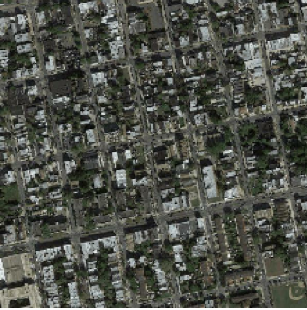
\includegraphics[width=\linewidth]{images/Pix2PixResults/Eingabe-Bild.png}
	\end{subfigure}
	\begin{subfigure}[t]{.14\textwidth}
		\centering
		\caption*{Ausgabe}
		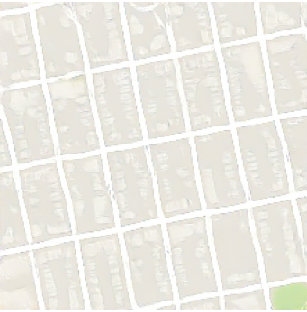
\includegraphics[width=\linewidth]{images/Pix2PixResults/Generiertes-Bild.png}
	\end{subfigure}
	\begin{subfigure}[t]{.14\textwidth}
		\centering
		\caption*{Zielbild}
		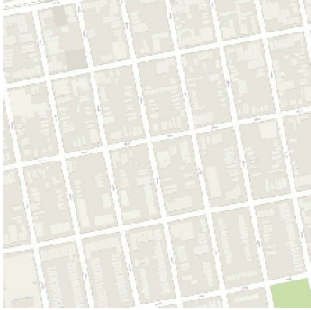
\includegraphics[width=\linewidth]{images/Pix2PixResults/Ziel-Bild.png}
	\end{subfigure}
	\hfill
	\begin{subfigure}[t]{.14\textwidth}
		\centering
		\caption*{Eingabe}
		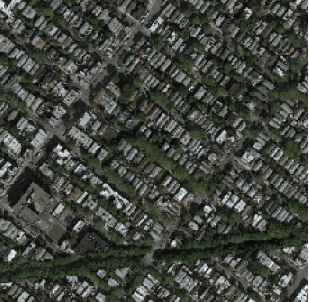
\includegraphics[width=\linewidth]{images/Pix2PixResults/Eingabe-Bild2.png}
	\end{subfigure}
	\begin{subfigure}[t]{.14\textwidth}
		\centering
		\caption*{Ausgabe}
		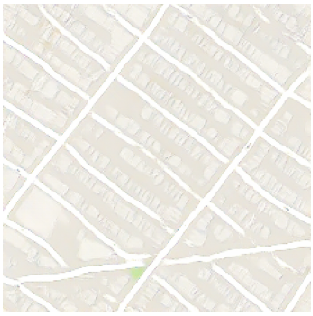
\includegraphics[width=\linewidth]{images/Pix2PixResults/Generiertes-Bild2.png}
	\end{subfigure}
	\begin{subfigure}[t]{.14\textwidth}
		\centering
		\caption*{Zielbild}
		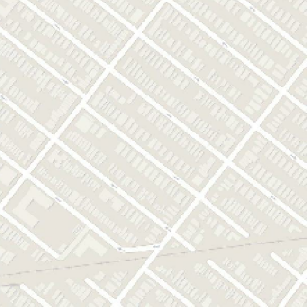
\includegraphics[width=\linewidth]{images/Pix2PixResults/Ziel-Bild2.png}
	\end{subfigure}
	\label{fig:StreePic}
\end{figure}

Die Evaluierung der Trainingsresultate des Pix2Pix-Modells basiert auf einer Analyse der 100 durchgeführten Trainingsepochen. Während des Durchlaufs dieser Epochen wurden spezifische Metriken wie Generator- und Diskriminator-Verluste sowie Diskriminator-Genauigkeit und der Structural Similarity Index Measure (SSIM) überwacht.\newline

Der Verlust des Generator beginnt bei 14.44 in der ersten Epoche und sinkt dann kontinuierlich ab, was auf ein erfolgreiches Lernen hinweist. Es gibt Schwankungen im Verlauf des Trainings, aber insgesamt zeigt sich ein Abwärtstrend, was darauf hindeutet, dass der Generator zunehmend besser in der Lage ist, glaubwürdige Bilder zu erzeugen.\newline
Der Diskriminator-Verlust beginnt bei 0.93 und zeigt eine leichte Abnahme über die Zeit. Dies deutet darauf hin, dass der Diskriminator im Laufe des Trainings besser darin wird, echte Bilder von gefälschten zu unterscheiden. Mit der Erhöhung von $\lambda$ bei Epoche 80 fokussiert sich der Generator mehr darauf, die exakten Pixelwerte des Zielbildes nachzubilden, dadurch muss sich der Diskriminator an die neuen Unterschiede zwischen realen und generierten Bildern anpassen. Aus diesem Grund kann dies anfänglich zu einem Anstieg des Diskriminatorverlusts führen, da seine Aufgabe nun schwieriger wird. In Abbildung \ref{fig:Verlustkurve 0-100} wird die Entwicklung der Verlustfunktionen nochmal grafisch dargestellt.
\begin{figure}[h]
	\centering
	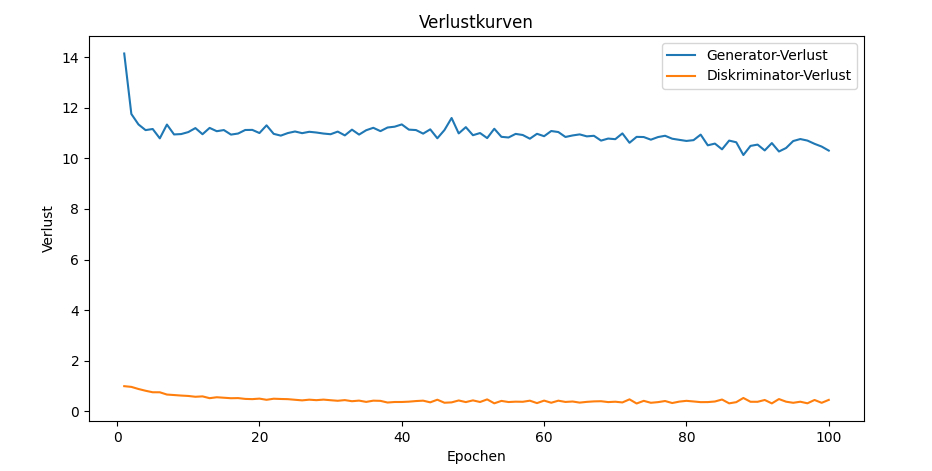
\includegraphics[width=1.0\textwidth]{images/Pix2PixResults/Verlust0-100.png}
	\caption{Generator- und Diskriminatorverlust des Trainingsdurchlaufs mit 100 Epochen, eigene Erstellung mittels matplotlib.pyplot-Bibliothek }
	\label{fig:Verlustkurve 0-100}
\end{figure}
 \newpage

Die Analyse der Diskriminatorgenauigkeit im Trainingsverlauf zeigt einen Anstieg der Genauigkeit über 90$\%$ was weit über den Idealwert 50$\%$. Dies ist ein Anzeichen dafür das der Diskriminator möglicherweise zu effektiv darin geworden ist, generierte Bilder von realen zu unterscheiden. Dieser Wert ist ein Indikator dafür, dass der Diskriminator fast immer richtig liegt und könnte darauf hindeuten, dass der Generator nicht genügend Raum bekommt, um zu lernen und sich zu verbessern. Zusätzlich weisen die Schwankungen, wie in Abbildung \ref{fig:Genauigkeit 0-100} gezeigt, auf eine gewisse Inkonsistenz im Lernprozess hin.
\begin{figure}[h]
	\centering
	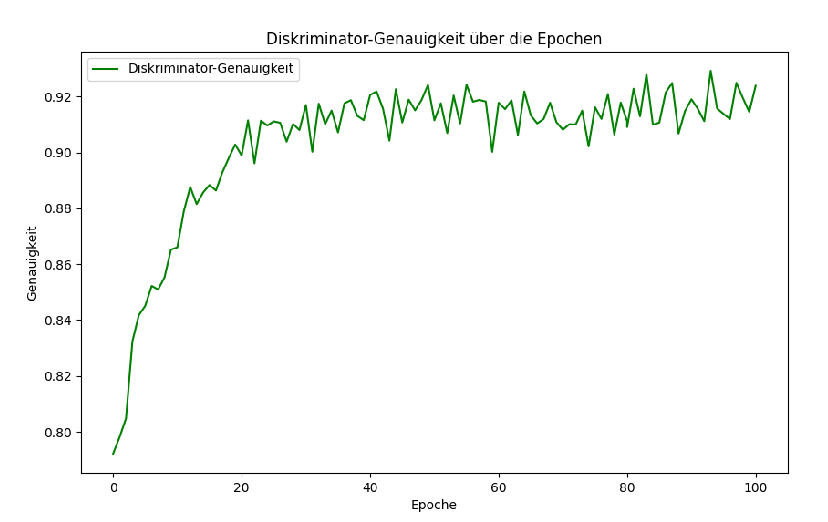
\includegraphics[width=1.0\textwidth]{images/Pix2PixResults/Genauigkeit0-100.png}
	\caption{Diskriminatorgenauigkeit des Trainingsdurchlaufs mit 100 Epochen, eigene Erstellung mittels matplotlib.pyplot-Bibliothek }
	\label{fig:Genauigkeit 0-100}
\end{figure}
 \newpage
Der SSIM-Score hatte anfänglich einen Wert von 0.5549 der allmählich anstieg, was auf eine Verbesserung der Bildqualität hindeutet, die der Generator im Laufe des Trainings erzielt. Dieser Trend ist ein positives Zeichen dafür, dass der Generator zunehmend besser darin wird, Bilder zu erzeugen, die den Zielbildern ähnlicher sind. Interessanterweise steigt der SSIM-Wert nicht kontinuierlich, wie in Abbildung \ref{fig:SSIM 0-100} zu sehen ist, sondern zeigt einige Schwankungen, was auf unterschiedliche Leitungen des Gnerators bei verschiedenen Bildern hinweist. Diese Inkonsistenzen könnten auf die Variabilität innerhalb des Trainingsdatensatzes oder auf die begrenzte Fähigkeit des Generator zurückzuführen sein bei bestimmten Strukturen wie beispielweise Grünflächen oder Wasser Probleme zu haben.\newline
Bemerkenswert ist der Anstieg des SSIM-Wertes nach der 80. Epoche, was zeitlich mit der Erhöhung des Lambda-Wertes von 100 auf 150 korreliert. Dies könnte darauf hindeuten, dass die Erhöhung des Lambda-Wertes dazu beigetragen hat, die Qualität der generierten Bilder in Bezug auf ihre strukturelle Ähnlichkeit zu verbessern. Der höhere SSIM-Wert in späteren Epochen könnte ein Indikator dafür sein, dass der Generator lernt, sich auf die wichtigen Aspekte der Bilder zu konzentrieren, die zur Ähnlichkeit mit den Zielbildern beitragen. 
\begin{figure}[h]
	\centering
	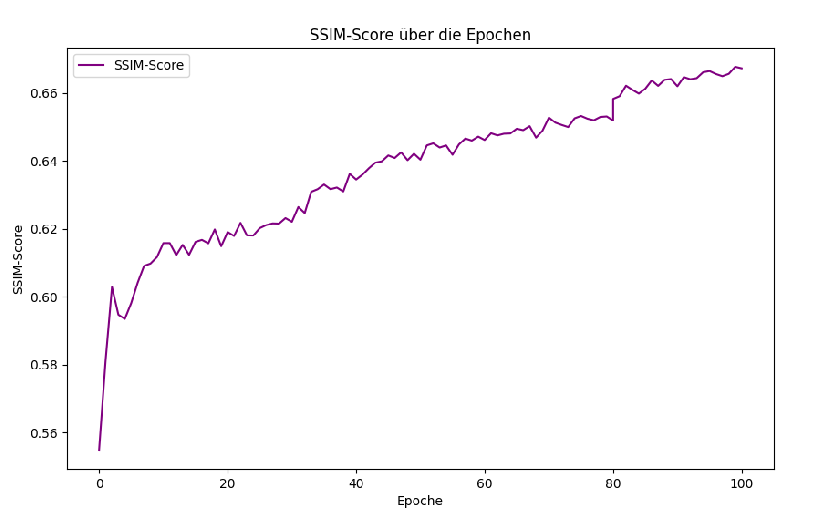
\includegraphics[width=1.0\textwidth]{images/Pix2PixResults/SSIM0-100.png}
	\caption{SSIM-Score des Trainingsdurchlaufs mit 100 Epochen, eigene Erstellung mittels matplotlib.pyplot-Bibliothek }
	\label{fig:SSIM 0-100}
\end{figure}

Das Pix2Pix GAN-Modell demonstriert seine Stärken in der Umwandlung von Satellitenbildern zu Karten, mit besonderer Kompetenz in der Darstellung von Straßenstrukturen. Trotzdem stößt es bei der Generierung komplexerer Elemente wie Grünflächen und Wasser auf Herausforderungen. Die Feinabstimmung der Hyperparameter, einschließlich einer geringen Batchgröße und einer spezifischen Anpassung des Lambda-Wertes, hat die Trainingseffizienz verbessert, was sich in einem erhöhten SSIM-Score niederschlägt. Allerdings weist die hohe Diskriminatorgenauigkeit von über 90$\%$ darauf hin, dass das Modell weiter optimiert werden muss, um ein Gleichgewicht zwischen Generator und Diskriminator zu erlangen. Hervorzuheben ist die signifikante Zeitersparnis durch die Verwendung einer GPU im Vergleich zur CPU: Während eine Epoche auf der CPU 320 Sekunden dauert, wird diese Zeit auf der GPU auf nur 20 Sekunden reduziert.
\newpage
\subsection{CycleGAN}
Die Datensätze $X$ (Karten) und $Y$ (Satellitenbilder) werden durch die Generatoren $G: X\rightarrow Y$ und $F: Y\rightarrow X$ sowie die Diskriminatoren $D_X$ und $D_Y$ repräsentiert, die jeweils darauf abzielen, Bilder in den Domänen $X$ und $Y$ zu unterscheiden. Die Hyperparameter basieren zunächst auf den in dem Originalpaper von Zhu ausgewählten Parametern und wurden anschließend durch explorative Anpassungen verfeinert.
\\\newline
Ein herausforderndes Problem, dem sich die Generatoren gegenübersehen, besteht in der Reproduktion feiner und detaillierter Strukturen. Insbesondere fällt auf, dass die Generatoren besser darin sind, Straßenlinien zu erzeugen, was auf die Dominanz von Straßen- und Häusermotiven in den Trainingsdaten zurückzuführen ist.
Die Vielfalt in den Bildern, wie Flüsse und Wälder, stellt hingegen eine größere Herausforderung dar. Die Generatoren haben Schwierigkeiten, die Struktur und Farbkodierung dieser Bereiche präzise zu erfassen. Häufig resultiert dies in der Generierung von Flächen mit ähnlicher Farbe wie Straßen, und es werden Versuche unternommen, basierend auf diesen großen Freiflächen kleine Straßen zu generieren.
\\\newline
Die Wahl der Lernrate erwies sich als kritisch, wobei die besten Ergebnisse bei einer Lernrate von $0,0002$ erzielt wurden. Diese Einstellung führte zu den höchsten SSIM-Werten und Diskriminator-Testgenauigkeiten. Insbesondere erzielte der Generator $F$ einen SSIM-Score von $0.592$, während der Generator $G$ einen Wert von $0.198$ erreichte. Die Diskriminatoren zeigten mit $50.1\%$ für $D_Y$ und $48,5\%$ für $D_X$ nahezu optimale Genauigkeiten. Trotz der zunächst hoch erscheinenden visuellen Ähnlichkeit zwischen den generierten Satellitenbildern zeigte eine genauere Analyse, dass kleinere Strukturen im generierten Bild fehlten. Dies spiegelte sich in den vergleichsweise niedrigen SSIM-Wert wider.



\begin{figure}
  \begin{subfigure}[t]{.3\textwidth}
    \centering
    \caption{Input}
    \includegraphics[width=\linewidth]{example-image-a}
  \end{subfigure}
  \hfill
  \begin{subfigure}[t]{.3\textwidth}
    \centering
    \caption{Output}
    \includegraphics[width=\linewidth]{example-image-b}
  \end{subfigure}
  \hfill
  \begin{subfigure}[t]{.3\textwidth}
    \centering
    \caption{Differenzbild}
    \includegraphics[width=\linewidth]{example-image-b}
  \end{subfigure}

  \medskip

  \begin{subfigure}[t]{.3\textwidth}
    \centering
    \includegraphics[width=\linewidth]{example-image-a}
  \end{subfigure}
  \hfill
  \begin{subfigure}[t]{.3\textwidth}
    \centering
    \includegraphics[width=\linewidth]{example-image-b}
  \end{subfigure}
  \hfill
  \begin{subfigure}[t]{.3\textwidth}
    \centering
    \includegraphics[width=\linewidth]{example-image-b}
  \end{subfigure}
  \caption{Testergebnisse nach dem Training mit $\lambda=120$, Lernrate $=0.0002$ und $100$ Epochen}
  \label{evaluation:cycleGan_Testergebnisse}
\end{figure}

\begin{figure}
  \begin{subfigure}[t]{.24\textwidth}
    \centering
    \includegraphics[width=\linewidth]{example-image-a}
    \caption{(a) Generator-Verlust}
  \end{subfigure}
  \begin{subfigure}[t]{.24\textwidth}
    \centering
    \includegraphics[width=\linewidth]{example-image-b}
    \caption{(b) Diskriminator-Metriken}
  \end{subfigure}
  \begin{subfigure}[t]{.24\textwidth}
    \centering
    \includegraphics[width=\linewidth]{example-image-b}
    \caption{(c) SSIM-Score}
  \end{subfigure}
  \begin{subfigure}[t]{.24\textwidth}
    \centering
    \includegraphics[width=\linewidth]{example-image-b}
    \caption{(d) SSIM-Score Zyklus}
  \end{subfigure}

  \caption{Metriken nach dem Training mit $\lambda=120$, Lernrate $=0.0002$ und $100$ Epochen}
  \label{evaluation:cycleGan_Metriken}
\end{figure}


Ebenso zeigten die Bilder bei einem Gewichtungsfaktor von $\lambda = 120$ die besten Resultate, sowohl basierend auf visueller Beurteilung als auch auf dem SSIM-Score (\ref{evaluation:cycleGan_Testergebnisse}). Dieser spezifische Wert für $\lambda$ führte zu generierten Bildern, deren Signal-Rausch-Verhältnis (SNR) entweder besser oder nahezu dem des Originalbildes entspricht. Der SNR-Wert gibt dabei das Verhältnis zwischen dem Signal, repräsentiert durch die relevanten Bildinformationen, und dem Rauschen, repräsentiert durch unerwünschte Störungen, an. In diesem Zusammenhang zeigt ein höherer SNR-Wert eine bessere Qualität und Klarheit der generierten Bilder im Vergleich zu Rauschen.
\\\newline
Trotz dieser Erfolge bleibt das Training instabil, und es besteht die Möglichkeit eines Modekollapses. Die Generatoren zeigen Anzeichen eines exponentiellen Verfalls in ihren Verlustkurven, während der SSIM-Score nur langsam ansteigt. Dies deutet darauf hin, dass die Generatoren zwar ihre Verluste minimieren, jedoch möglicherweise nicht die gewünschte visuelle Qualität erreichen (\ref{evaluation:cycleGan_Metriken}).

\begin{figure}
  \begin{subfigure}[t]{.2\textwidth}
    \caption{Input}
    \centering
    \includegraphics[width=\linewidth]{example-image-a}
  \end{subfigure}
  \begin{subfigure}[t]{.2\textwidth}
    \caption{Output}
    \centering
    \includegraphics[width=\linewidth]{example-image-b}
  \end{subfigure}
  \hfill
  \begin{subfigure}[t]{.2\textwidth}
    \caption{Input}
    \centering
    \includegraphics[width=\linewidth]{example-image-a}
  \end{subfigure}
  \begin{subfigure}[t]{.2\textwidth}
    \caption{Output}
    \centering
    \includegraphics[width=\linewidth]{example-image-b}
  \end{subfigure}

  \medskip

  \begin{subfigure}[t]{.2\textwidth}
    \centering
    \includegraphics[width=\linewidth]{example-image-a}
  \end{subfigure}
  \begin{subfigure}[t]{.2\textwidth}
    \centering
    \includegraphics[width=\linewidth]{example-image-b}
  \end{subfigure}
  \hfill
  \begin{subfigure}[t]{.2\textwidth}
    \centering
    \includegraphics[width=\linewidth]{example-image-a}
  \end{subfigure}
  \begin{subfigure}[t]{.2\textwidth}
    \centering
    \includegraphics[width=\linewidth]{example-image-b}
  \end{subfigure}

  \medskip

  \begin{subfigure}[t]{.2\textwidth}
    \centering
    \includegraphics[width=\linewidth]{example-image-a}
  \end{subfigure}
  \begin{subfigure}[t]{.2\textwidth}
    \centering
    \includegraphics[width=\linewidth]{example-image-b}
  \end{subfigure}
  \hfill
  \begin{subfigure}[t]{.2\textwidth}
    \centering
    \includegraphics[width=\linewidth]{example-image-a}
  \end{subfigure}
  \begin{subfigure}[t]{.2\textwidth}
    \centering
    \includegraphics[width=\linewidth]{example-image-b}
  \end{subfigure}

  \medskip

  \begin{subfigure}[t]{.2\textwidth}
    \centering
    \includegraphics[width=\linewidth]{example-image-a}
  \end{subfigure}
  \begin{subfigure}[t]{.2\textwidth}
    \centering
    \includegraphics[width=\linewidth]{example-image-b}
  \end{subfigure}
  \hfill
  \begin{subfigure}[t]{.2\textwidth}
    \centering
    \includegraphics[width=\linewidth]{example-image-a}
  \end{subfigure}
  \begin{subfigure}[t]{.2\textwidth}
    \centering
    \includegraphics[width=\linewidth]{example-image-b}
  \end{subfigure}
  \caption{Beste Ergebnisse des Trainings}

\end{figure}


Die generierten Bilder weisen bereits zu diesem Zeitpunkt eine grobe visuelle Ähnlichkeit mit der Struktur des zugrunde liegenden Originalbildes auf und zeigen nur minimale Variationen. Allerdings wird durch den SSIM-Score deutlich, dass die Generatoren Schwierigkeiten haben, bedeutende Verbesserungen hinsichtlich feinerer Details und Farbübereinstimmungen zu erzielen. Diese lassen sich auch visuell in den Differenzbilder, die mit Hilfe eines Histogrammsausgleich kontrastverstärkt wurden, erkennen. Helle Bereiche in diesen Differenzbildern stellen dabei größere Unterschiede dar. Dabei sammeln sich helle Bereiche vor allem bei den kleinen pixelweisen Details an, sowie bei unterschiedlichen Farbkodierungen. Ein konkretes Beispiel ist in Abbildung \ref{evaluation:cycleGan_Testergebnisse} zu sehen.
\\
Insbesondere in den frühen Epochen sind die Generatoren nicht in der Lage, Straßenlinien zuverlässig als gerade Linien zu generieren. Diese Schwächen verbessern sich im Laufe längerer Trainingszeiten, wobei bereits nach etwa 300 Epochen relativ konsistente, gerade Linien erzeugt werden.
\\\newline
Die Analyse des SSIM-Scores im Kontext der Zyklusübersetzung offenbart eine exponentielle Zunahme. Diese Beobachtung legt nahe, dass der Zykluskonsistenz-Verlust einen erheblichen Einfluss auf das Training ausübt. Die exponentielle Steigerung des SSIM-Scores deutet darauf hin, dass die Konsistenz zwischen den Original- und zurückübersetzten Bildern im Laufe der Zeit kontinuierlich zunimmt. Dies könnte auf eine fortlaufende Verbesserung der Generatoren hinsichtlich ihrer Fähigkeit zur Zyklusübersetzung hindeuten. Insgesamt erreichen die SSIM-Scores für die Zyklusübersetzung Werte von $80\%$ für $Y$ und $90\%$ für $X$ (\ref{evaluation:cycleGan_Metriken}).

\begin{table}
\centering
\begin{tabular}{|l|l|l|l|l|l|l|l|l|l|l|l|l|l|l|}
\hline
\textbf{Lambda} &
  \textbf{Epoche} &
  \textbf{Lernrate} &
  \textbf{\begin{tabular}[c]{@{}l@{}}$D_Y$ \\ Tr-Acc\end{tabular}} &
  \textbf{\begin{tabular}[c]{@{}l@{}}$D_X$ \\ Tr-Acc\end{tabular}} &
  \textbf{\begin{tabular}[c]{@{}l@{}}$D_Y$ \\ Te-Acc\end{tabular}} &
  \textbf{\begin{tabular}[c]{@{}l@{}}$D_X$ \\ Te-Acc\end{tabular}} \\ \hline
120 & 100 & 0.000025 & 0.549 & 0.494 & 0.307 & 0.497   \\ \hline
120 & 100 & 0.00005  & 0.537 & 0.491 & 0.321 & 0.489 \\ \hline
120 & 100 & 0.0001   & 0.519 & 0.490 & 0.418 & 0.485 \\ \hline
120 & 100 & 0.0002   & 0.518 & 0.495 & 0.501 & 0.485 \\ \hline
120 & 100 & 0.0004   & 0.516 & 0.487 & 0.462 & 0.496 \\ \hline
100 & 100 & 0.0002   & 0.521 & 0.491 & 0.527 & 0.481   \\ \hline
140 & 100 & 0.0002   & 0.562 & 0.492 & 0.544 & 0.469 \\ \hline
100 & 300 & 0.0002   & 0.51  & 0.484 & 0.47  & 0.676 \\ \hline
120 & 300 & 0.0002   & 0.508 & 0.495 & 0.468 & 0.709  \\ \hline
\end{tabular}
\caption{CycleGAN Ergebnisse unter verschiedenen Hyperparameter Teil1}
\label{evaluation:cycleGan_table1}
\end{table}

\begin{table}
\centering
\begin{tabular}{|l|l|l|l|l|l|l|l|l|l|l|l|l|l|l|}
\hline
\textbf{\begin{tabular}[c]{@{}l@{}}$F$\\ Loss\end{tabular}} &
\textbf{\begin{tabular}[c]{@{}l@{}}$G$\\ Loss\end{tabular}} &
  \textbf{\begin{tabular}[c]{@{}l@{}}$X$ \\ SSIM\end{tabular}} &
  \textbf{\begin{tabular}[c]{@{}l@{}}$Y$ \\SSIM \end{tabular}} &
  \textbf{\begin{tabular}[c]{@{}l@{}}$X$\\Z-SSIM\end{tabular}} &
  \textbf{\begin{tabular}[c]{@{}l@{}}$Y$ \\ Z-SSIM\end{tabular}} &
  \textbf{\begin{tabular}[c]{@{}l@{}}$X$\\SNR \end{tabular}} &
  \textbf{\begin{tabular}[c]{@{}l@{}}$Y$\\SNR\end{tabular}} \\ \hline
53.113 & 22.556 & 0.545 & 0.191 & 0.895 & 0.831 & -2.991 & 0.228  \\ \hline
44.626 & 20.417 & 0.541 & 0.191 & 0.916 & 0.836 & -0.589 & 1.071  \\ \hline
44.376 & 21.943 & 0.580 & 0.194 & 0.935 & 0.842 & -4.604 & 1.367  \\ \hline
42.489 & 22.373 & 0.592 & 0.198 & 0.921 & 0.796 & -5.308 & 0.851  \\ \hline
46.972 & 28.175 & 0.585 & 0.209 & 0.856 & 0.602 &        &        \\ \hline
34.973 & 18.837 & 0.551 & 0.194 & 0.93  & 0.83  & -3.292 & 1.261  \\ \hline
13.048 & 6.842  & 0.510 & 0.179 & 0.513 & 0.409 & -2.087 & 1.005  \\ \hline
34.881 & 20.899 & 0.577 & 0.191 & 0.931 & 0.756 & -2.705 & 1.373  \\ \hline
46.652 & 26.360 & 0.585 & 0.207 & 0.901 & 0.707 & 1.248  & -3.409 \\ \hline
\end{tabular}
\caption{CycleGAN Ergebnisse unter verschiedenen Hyperparameter Teil2}
\label{evaluation:cycleGan_table2}
\end{table}


Im Kontrast dazu bleibt die Genauigkeit der Diskriminatoren für Trainingsdaten stabil bei etwa $50\%$. Jedoch zeigen sich erhebliche Schwankungen je nach Epoche für die Testdaten, insbesondere für $D_Y$. Dies legt nahe, dass die Diskriminatoren möglicherweise Schwierigkeiten haben, mit neuen, nicht trainierten Daten umzugehen. Diese Schwankungen könnten auf Überanpassung oder eine mangelnde Generalisierungsfähigkeit des Modells hinweisen, trotz der implementierten Maßnahmen wie dem Hinzufügen von Rauschen und Dropout-Schichten (\ref{evaluation:cycleGan_Metriken}).
\\\newline
Die Laufzeit des Trainings spiegelt die Komplexität der Modelle wider, insbesondere auf der GPU, wo jede Epoche im Durchschnitt etwa 2 Minuten dauert. Im Vergleich dazu benötigt die CPU, selbst nach einer Reduzierung der Residualblöcke auf einen Block, rund 6 Minuten pro Epoche. Die Nutzung von Instanznormalisierung trägt zur beschleunigten Konvergenz und Verbesserung der Laufzeit bei. Zudem zeigt sich, dass die Verwendung von Residualblöcken eine bessere Laufzeit ermöglicht im Vergleich zu Generatoren mit zusätzlichen Schichten. 
\\\newline
Insgesamt zeigt die Evaluation, dass das CycleGAN-Modell trotz einiger Herausforderungen in der Generierung von detaillierten Strukturen und der Generalisierung auf neue Daten vielversprechende Ergebnisse erzielt.



\newpage
\section{Vergleich von Pix2Pix und CycleGAN}
Pix2Pix und CycleGAN sind beides Modelle von Generative Adversarial Networks, die für Bild-zu-Bild-Übersetzungen eingesetzt werden, jedoch unterscheiden sie sich wesentlich in ihrer Methodik und den Anwendungsbereichen aufgrund ihrer strukturellen Unterschiede.
\\\newline
Die Pix2Pix-Architektur verwendet typischerweise einen U-Net-basierten Generator und einen PatchGAN-Diskriminator, der auf die einzelnen Bildabschnitte einwirkt, um festzustellen, ob sie echt oder gefälscht sind. Diese Architektur ermöglicht eine effektivere Erfassung hochauflösender Details. 
Der Diskriminator von CycleGAN basiert ebenfalls auf PatchGAN, verwendet jedoch Instanznormalisierung anstelle von Batchnormalisierung. Ein wesentlicher Unterschied besteht in den Generatoren. Diese basieren auf dem ResNet-Ansatz und erweitern Pix2Pix um einen Zykluskonsistenzverlust. Dieser stellt sicher, dass das Eingabebild in die Zieldomäne übersetzt und anschließend wieder in die Ursprungsdomäne zurückübersetzt wird, ohne dass der ursprüngliche Inhalt verloren geht. Diese bidirektionale Struktur soll helfen, die Mode-Kollapse zu vermeiden, und stellt sicher, dass der Generator vielfältige Ausgaben erzeugt.
\\\newline
Pix2Pix benötigt paarweise Trainingsdaten. Das bedeutet, dass jedes Trainingsbeispiel aus einem korrespondierenden Bildpaar, einem Eingabe- und einem Zielbild, besteht. Daher eignet sich das Pix2Pix-Modell besonders für Aufgaben, bei denen eine strukturierte und koordinierte Beziehung zwischen Eingabe- und Ausgabebild besteht, wie bei der Umwandlung von Satellitenbildern in Karten oder beim Einfärben von Schwarzweißfotos. 
Im Gegensatz dazu ist CycleGAN für die Arbeit mit ungepaarten Trainingsdaten konzipiert, die das Lernen von Übersetzungen ohne eine Eins-zu-Eins-Zuordnung zwischen Quell- und Zielbildern ermöglichen. Dies ist besonders nützlich für Stiltransformationen, beispielsweise für Pferde in Zebras oder Äpfel in Orangen, für die es keine gepaarten Beispiele gibt. Des Weiteren wird eine größere Flexibilität und Unabhängigkeit spezifischer Datensätze ermöglicht.
\\\newline
Die Evaluierung zeigt die wesentlichen Stärken und Schwächen der beiden GAN-Architekturen. Beide haben mit einer Lernrate von $0,0002$ gute Ergebnisse erzielt. Der $\lambda$-Wert variiert bei Pix2Pix, während bei CycleGAN ein konstanter $\lambda$-Wert verwendet wird.
\\
Es stellt sich heraus, dass beide Generatoren effizient sind, wenn es darum geht, Straßenlinien zu erzeugen, aber dass es für beide schwierig ist, die Struktur und Farbkodierung von vielfältigeren Bildern, wie Flüssen und Wäldern, genau zu erfassen. Außerdem steigt der SSIM-Wert von CycleGAN exponentiell mit großen Ausreißern, während der SSIM-Wert von Pix2Pix relativ linear mit der Zeit ansteigt. Dies spiegelt sich auch in den Verlusten der Generatoren und Diskriminatoren wider. Bei CycleGAN ist die Abnahme exponentiell. Bei Pix2Pix ist sie linear. 
Pix2Pix zeigt insbesondere eine große Verbesserung der Genauigkeit des Diskriminators auf den Trainingsdaten, die nach einigen Epochen $90\%$ übersteigt. Im Gegensatz dazu bleibt die Genauigkeit des CycleGAN Diskriminators konstant bei $50\%$, was als optimal angesehen wird. Die Genauigkeit der Testdaten spiegelt dies teilweise wider.
Die Testgenauigkeit bei Pix2Pix ist mit $37.5\%$ dagegen niedrig, obwohl die Trainingsgenauigkeit im Vergleich sehr hoch ist. Dies und die großen Schwankungen bei CycleGAN können auf eine Überanpassung der Diskriminatoren zurückgeführt werden.
\\

\begin{figure}
	\centering
	\begin{subfigure}[t]{.2\textwidth}
	  \caption*{Input}
	  \centering
	  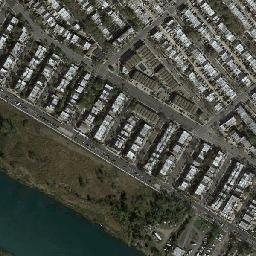
\includegraphics[width=\linewidth]{images/cycleGanResults/Satelite6_Or_Ld120_E100_Lr0002.jpg}
	\end{subfigure}
	\begin{subfigure}[t]{.2\textwidth}
	  \caption*{Pix2Pix}
	  \centering
	  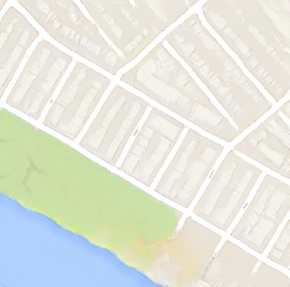
\includegraphics[width=\linewidth]{images/Vergleich/p3.png}
	\end{subfigure}
	\begin{subfigure}[t]{.2\textwidth}
	  \caption*{CycleGAN}
	  \centering
	  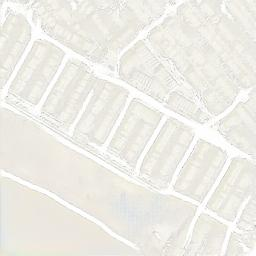
\includegraphics[width=\linewidth]{images/cycleGanResults/Maps6Ld120_E100_Lr0002.jpg}
	\end{subfigure}
	\begin{subfigure}[t]{.2\textwidth}
	  \caption*{Output}
	  \centering
	  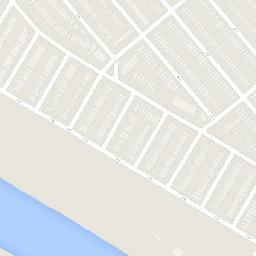
\includegraphics[width=\linewidth]{images/cycleGanResults/Maps6_Or_Ld120_E100_Lr0002.jpg}
	\end{subfigure}
  
	\medskip

	\begin{subfigure}[t]{.2\textwidth}
		\centering
		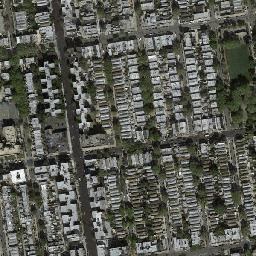
\includegraphics[width=\linewidth]{images/cycleGanResults/Satelite19_Or_Ld120_E100_Lr0002.jpg}
	  \end{subfigure}
	  \begin{subfigure}[t]{.2\textwidth}
		\centering
		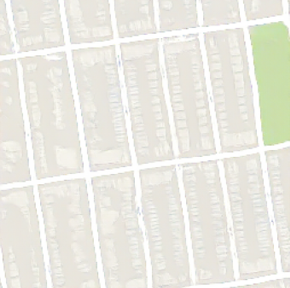
\includegraphics[width=\linewidth]{images/Vergleich/p2.png}
	  \end{subfigure}
	  \begin{subfigure}[t]{.2\textwidth}
		\centering
		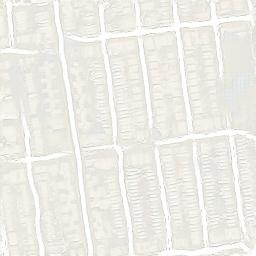
\includegraphics[width=\linewidth]{images/cycleGanResults/Maps19Ld120_E100_Lr0002.jpg}
	  \end{subfigure}
	  \begin{subfigure}[t]{.2\textwidth}
		\centering
		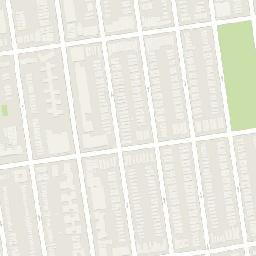
\includegraphics[width=\linewidth]{images/cycleGanResults/Maps19_Or_Ld120_E100_Lr0002.jpg}
	  \end{subfigure}
	
	\medskip

	\begin{subfigure}[t]{.2\textwidth}
		\centering
		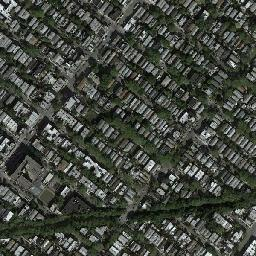
\includegraphics[width=\linewidth]{images/Vergleich/Satelite12.jpg}
	  \end{subfigure}
	  \begin{subfigure}[t]{.2\textwidth}
		\centering
		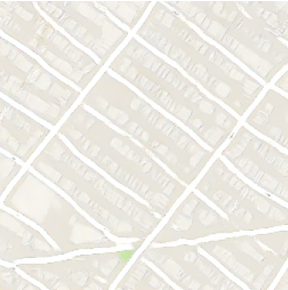
\includegraphics[width=\linewidth]{images/Vergleich/p4.png}
	  \end{subfigure}
	  \begin{subfigure}[t]{.2\textwidth}
		\centering
		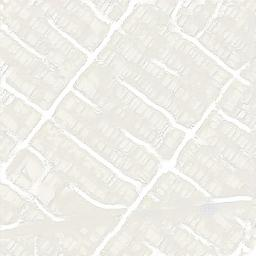
\includegraphics[width=\linewidth]{images/Vergleich/Maps12_t.jpg}
	  \end{subfigure}
	  \begin{subfigure}[t]{.2\textwidth}
		\centering
		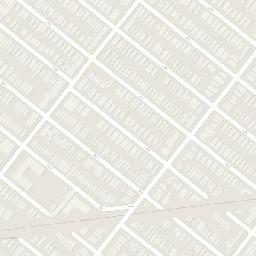
\includegraphics[width=\linewidth]{images/Vergleich/Maps12.jpg}
	  \end{subfigure}
	
	\medskip

	\begin{subfigure}[t]{.2\textwidth}
		\centering
		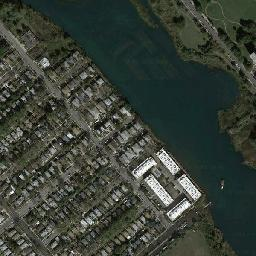
\includegraphics[width=\linewidth]{images/Vergleich/Satelite17.jpg}
	  \end{subfigure}
	  \begin{subfigure}[t]{.2\textwidth}
		\centering
		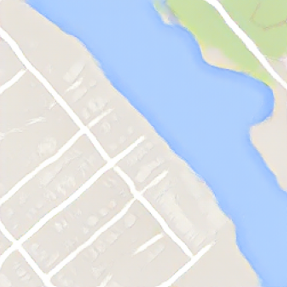
\includegraphics[width=\linewidth]{images/Vergleich/p11.png}
	  \end{subfigure}
	  \begin{subfigure}[t]{.2\textwidth}
		\centering
		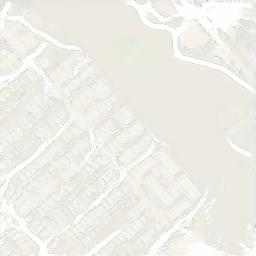
\includegraphics[width=\linewidth]{images/Vergleich/Maps17_t.jpg}
	  \end{subfigure}
	  \begin{subfigure}[t]{.2\textwidth}
		\centering
		\includegraphics[width=\linewidth]{images/Vergleich/Maps12.jpg}
	  \end{subfigure}
  
	\caption{Vergleich der Ergebnisse von Pix2Pix und CycleGAN}
  
  \end{figure}




Des Weiteren ist die Komplexität der Pix2Pix-Architektur aufgrund der 6-mal schnelleren Laufzeit geringer. Darüber hinaus wurde festgestellt, dass die Anpassung der Hyperparameter und die Stabilität gegenüber Mode-Kollapse bei CycleGAN schwieriger sind als bei Pix2Pix.
\\\newline
Aufgrund der direkten Korrespondenz zwischen Eingangs- und Ausgangsbildern zeigt Pix2Pix bessere Tendenzen bei der Projektion von Farbkodierungen als CycleGAN. Letzteres hat bereits große Schwierigkeiten, die richtige Stelle für die Farbkodierung zu finden. 
Andererseits ist es mit den beiden Generatoren von CycleGAN möglich, nach dem Training beide Bilddomänen abzubilden, während Pix2Pix auf die Abbildung nur einer Bilddomäne beschränkt ist. Die Wahl zwischen Pix2Pix und CycleGAN hängt daher stark von den verfügbaren Daten und den spezifischen Anforderungen der jeweiligen Aufgabe ab.